% Plantilla latex para protocolo de tesis de posgrado en la 
% Facultad de Ingeniería, Universidad Autónoma de Querétaro
%
% @author {Gerardo Hernández-Nava, Enrique Mena-Camilo, Sheila Leyva-López}
% @email {gerardohn.uam@gmail.com, enriquemece97@gmail.com, sheileyva29@gmail.com}
% @year 2022
% @version 1.0
% @license CC-BY-NC
%
% Se agradecen sus comentarios, contribuciones, 
% reporte de bugs y la difusión de esta plantilla


\documentclass[12pt, letterpaper, spanish, twoside]{article}
\AddToHook{cmd/section/before}{\newpage}
\usepackage{./common/UAQ}
\usepackage{graphicx} % Required for inserting images
\usepackage{pdflscape}
\usepackage[utf8]{inputenc}
\usepackage{subfig}
\usepackage{amsmath}
%\usepackage[spanish,es-tabla]{babel}
\usepackage{float}
\usepackage{geometry}
\usepackage{longtable}
\usepackage{enumitem} % Para ajustar listas dentro de tablas
\usepackage{url}
\usepackage{tocloft}
\usepackage[backend=biber,style=ieee]{biblatex}
\addbibresource{ref.bib}
\graphicspath{{./figures/}}
\bibliography{ref.bib}
\renewcommand{\thesubsection}{\thesection.\arabic{subsection}}
\renewcommand{\thesubsubsection}{\thesubsection.\arabic{subsubsection}}
\renewcommand{\cftsecnumwidth}{3em} 
\renewcommand{\cftsubsecnumwidth}{3em}  % Para \subsection

\begin{document}

% Fondo de portada
\backgroundsetup{
	scale = 1,
	angle = 0,
	opacity = 1,
	contents = {
		
\includegraphics[width=\paperwidth]{../figures/CoverBackground.pdf}
	}
}

\begin{titlepage}

\vspace*{10cm}
{\huge \bfseries \textcolor{RojoUAQ}{Localización avanzada de fuentes de señales de electroencefalograma mediante técnicas de computación avanzada }\\[1cm] }

\begin{center}
	\noindent
	\begin{minipage}{0.4\textwidth}
	\begin{flushleft} \large
	\emph{Estudiante:}\\
	Ing. Daniel Eduardo González Alvarado
	\end{flushleft}
	\end{minipage}	
	\begin{minipage}{0.4\textwidth}
	\begin{flushright} \large
	\emph{Director:} \\
	Dr. Takacs Andras \\[1.5cm]
	\end{flushright}
	\end{minipage}
    
	\vfill
    
	{\large \today}
\end{center}
\end{titlepage}


\backgroundsetup{
	scale = 1,
	angle = 0,
	opacity = 1,
	contents = {
		
\includegraphics[width=\paperwidth]{../figures/BodyBackground.pdf}
	}
}

\pagenumbering{\Roman}
\setlength{\cftsecnumwidth}{3em} %Se cambia el espacio entre el item y el nombre de la seccion
\setlength{\cftsubsecindent}{1.3cm}
\setlength{\cftsubsubsecindent}{2.4cm}
\tableofcontents

\pagenumbering{arabic}
\section*{Datos generales}
\addcontentsline{toc}{section}{Datos generales}
\begin{itemize}
	\item Título del proyecto de Tesis: Localización avanzada de fuentes de señales de electroencefalograma mediante técnicas de computación avanzada 
	\item Nombre del alumno: Daniel Eduardo González Alvarado
	\item Número de expediente: 338044
	\item Programa de Estudios a realizar: Maestría
	\item Director de Tesis: Andras Takacs
	\item Secretario: Hebert Luis Hernández Montiel
	\item Vocal: Marcos Romo
	\item Lugar donde se realizará la investigación: UAQ campus Aeropuerto
	\item Línea de investigación: Científica
	\item Tipo de investigación: Tecnológica 
	\item Horario de trabajo: 8:00 - 17:00 hrs
\end{itemize}

\section{Introducción}

% 150-200 Palabras
% Hacer hasta el Final
        Usando mediciones de voltaje en el cuero cabelludo (EEG por sus siglas en ingles) o mediciones de campo magnético en la superficie de la cabeza (MEG por sus siglas en ingles) se busca estimar su fuente de emisión. Esto implica trabajar hacia atrás del sensor (Problema Inverso) para determinar las fuentes intercraneales esto nos proveerá con características espacio-temporales de la fuente neuronal.

    \subsection{Métodos Actuales}
    Los métodos actuales de localización de fuentes cerebrales a partir de señales de EEG o MEG se dividen principalmente en dos grandes categorías: los modelos paramétricos, que suponen un número reducido y definido de fuentes activas (como el dipole fitting y MUSIC), y los modelos distribuidos, que estiman una distribución continua de corriente en el volumen cerebral (como MNE, LORETA, sLORETA, VARETA y LAURA). Estos enfoques han permitido importantes avances en el análisis funcional del cerebro, especialmente en aplicaciones clínicas como la epilepsia o la neurorehabilitación.

    Sin embargo, todos estos métodos comparten una dificultad inherente: el problema inverso es fundamentalmente mal condicionado. Es decir, existen múltiples configuraciones internas del cerebro que pueden generar las mismas señales observadas en la superficie. Esta ambigüedad limita la precisión espacial y temporal de las estimaciones y requiere incorporar supuestos o restricciones adicionales, lo cual puede introducir sesgos o reducir la generalización del modelo. Resolver esta problemática sigue siendo uno de los principales desafíos en el campo de la neuroimagen no invasiva.

\section{Antecedentes}
% 4 Pags (Maximo 5)
% Investigacion de Fuentes Legitimas
% Se escribe en Forma de reseña historica
 %Contextualización.
 %Identificación de brechas en el conocimiento.
 %Fundamentación teórica mínima necesaria para comprender el tema.
 %Apoyo metodológico.
 %Citar fuentes


La electroencefalografía (EEG por sus siglas en ingles) y la magnetoencefalografía (MEG por sus siglas en ingles) son técnicas no invasivas que registran la actividad eléctrica y magnética del cerebro desde el cuero cabelludo o fuera de la cabeza\cite{Asadzadeh2020}. A diferencia de otras modalidades de neuroimagen con alta resolución espacial (como la Imagen por Resonancia Magnética Funcional), el EEG y la MEG destacan por su extraordinaria resolución temporal a escala de milisegundos. Sin embargo, determinar la ubicación tridimensional de las fuentes neuronales que generan estas señales registradas en la superficie es un desafío inherentemente difícil, conocido como el problema inverso\cite{Hamalainen1994}. Este problema es fundamentalmente mal condicionado y no tiene una solución única sin incorporar suposiciones o restricciones adicionales. La búsqueda de métodos precisos para resolver este problema ha sido un área activa de investigación durante décadas, crucial para comprender la organización funcional del cerebro y diagnosticar trastornos neurológicos como la epilepsia.

\subsection{Primeros Enfoques: Modelos de Dipolo Discreto}

Una de las primeras y más comunes estrategias para abordar el problema inverso fue asumir que las señales EEG/MEG son generadas por un número relativamente pequeño de fuentes focales, modeladas como dipolos de corriente. Este enfoque paramétrico busca estimar la ubicación, orientación y magnitud de estos dipolos discretos. Trabajos tempranos, propusieron el uso del principio clasificación múltiple de señales (MUSIC por sus siglas en ingles)\cite{Mosher1992} para identificar las ubicaciones de múltiples dipolos a partir de datos MEG espacio-temporales. Demostraron que el análisis de componentes principales (PCA por sus siglas en ingles) podía ajustarse a un modelo de dipolo simple y utilizaron algoritmos de optimización como el método Simplex para la localización. Posteriormente, refinaron esta idea con Recursive MUSIC\cite{Mosher1998RecursiveMUSIC}, un marco iterativo que construye modelos topográficos de orden superior para localizar fuentes con mayor precisión. Si bien los modelos de dipolo discreto pueden ser apropiados cuando las fuentes son realmente localizadas, pueden llevar a resultados engañosos si las suposiciones no se cumplen o si el número de fuentes es desconocido.

\subsection{El Surgimiento de las Soluciones Distribuidas}

Una alternativa a los modelos de dipolo discreto es estimar la actividad neuronal no solo en puntos focales, sino distribuida en todo el volumen cerebral o en la superficie cortical\cite{Michel2019}. Este enfoque, conocido como soluciones inversas distribuidas (DIS por sus siglas en ingles), busca calcular una distribución de densidad de corriente tridimensional. Para superar la no unicidad del problema inverso en este contexto, se introducen restricciones basadas en información a priori.

Un desarrollo significativo fue la introducción de las Estimaciones de Norma Mínima (MNE por sus siglas en ingles)\cite{Hamalainen1994}. Las MNE buscan la distribución de corriente que tiene la norma mínima (una medida de ``tamaño'' o ``energía'') entre todas las distribuciones posibles que explican los datos medidos. Aunque las MNE son soluciones lineales que no requieren suposiciones sobre dipolos discretos y resultan en distribuciones de corriente continuas, tienden a ``difuminar'' o extender las fuentes puntuales reales\cite{ValdesSosa2000}.

\subsection{Regularización y LORETA}

Para obtener soluciones únicas y fisiológicamente plausibles en los métodos distribuidos, se aplica la regularización, que incorpora conocimiento a priori sobre las propiedades de la solución deseada\cite{Michel2019}. Un avance crucial fue la Tomografía Electromagnética de Baja Resolución (LORETA por sus siglas en inglés)\cite{PascualMarqui1994}. LORETA calcula directamente una distribución de corriente en todo el volumen cerebral aplicando una restricción de suavidad espacial, basada en la suposición fisiológica de que las neuronas vecinas tienden a activarse sincrónicamente.

Posteriormente, en 2002 se desarrollo la Tomografía Electromagnética Cerebral de Baja Resolución Estandarizada (sLORETA por sus siglas en inglés)\cite{PascualMarqui2002}, una versión estandarizada de LORETA que aborda algunas de sus limitaciones y se ha vuelto muy popular por su simplicidad y precisión aceptable\cite{Pantazis2021}. A pesar de su éxito, sLORETA puede producir imágenes ruidosas o borrosas, lo que ha llevado a desarrollos como EHR-sLORETA para mejorar la resolución mediante umbralización automática.

Otros métodos como el Promedio Autorregresivo Local (LAURA por sus siglas en inglés) \cite{GraveDePeralta2004}, y la Tomografía Eléctrica y Magnética de Resolución Variable (VARETA por sus siglas en inglés)\cite{ValdesSosa2000}, también han ofrecido aproximaciones distribuidas usando restricciones biofísicas o regularización espacialmente variable.

\begin{table}[H]
\centering
\caption{Comparación de modelos distribuidos para localización de fuentes}
\begin{tabular}{|p{3cm}|p{3cm}|p{3.5cm}|p{3cm}|p{2.5cm}|}
\hline
\textbf{Modelo} & \textbf{Principio Teórico} & \textbf{Salida Generada} & \textbf{Ventajas / Limitaciones} & \textbf{Precisión} \\
\hline
MNE & Minimización de la norma de la corriente estimada & Mapa continuo de corriente sobre una malla cerebral & Rápido y simple; subestima fuentes profundas & $\sim$10--20 mm \cite{Grech2008} \\
\hline
LORETA & Regularización suave espacial & Imagen 3D con resolución baja-media & Mejora estabilidad y reduce ruido; resolución limitada & $\sim$7--15 mm \cite{Grech2008} \\
\hline
sLORETA & Densidad de corriente estandarizada (z-score) & Imagen precisa con menor error de localización & Alta precisión en profundidad; dependiente de normalización & $\sim$5--10 mm \cite{PascualMarqui2002} \\
\hline
VARETA & Enfoque bayesiano multiresolución & Tomografía cerebral con resolución adaptativa & Alta resolución espacial; complejidad computacional elevada & $\sim$5--10 mm \cite{BoschBayard2001} \\
\hline
LAURA & Regularización local autoregresiva & Distribución localizada con restricciones espaciales & Optimiza precisión local; sensible a configuración de parámetros & $\sim$5--10 mm \cite{GraveDePeralta2004} \\
\hline
Aprendizaje Profundo (CNN) & Redes profundas aprenden relaciones no lineales EEG-fuente & Mapa de actividad de fuentes & Alta precisión, depende de datos de entrenamiento & $\sim$5--10 mm \cite{Hecker2021CNN} \\
\hline
Hybrid DL + MNE/LORETA & Combina modelo físico con red neuronal & Mapa ajustado de localización de fuentes & Mayor robustez, requiere calibración & $\sim$4--7 mm \cite{Zhang2021HybridEEG} \\
\hline
\end{tabular}
\end{table}



\subsection{Filtros Espaciales (Beamformers)}

Otra familia importante de técnicas de localización de fuentes son los filtros espaciales o beamformers\cite{Zhang2023EEGReview}. Métodos como la Varianza Mínima con Restricciones Lineales (LCMV por sus siglas en inglés)\cite{Sun2022DeepNN}, construyen filtros espaciales que estiman la actividad de una fuente específica mientras suprimen la actividad de otras. Los beamformers representan una alternativa a los métodos de norma mínima\cite{Hincapie2016} y han demostrado ser útiles en la detección de fuentes interactuantes. Su rendimiento puede depender del preprocesamiento y la elección de parámetros\cite{Asadzadeh2020}.

\subsection{Integración Multimodal y Restricciones Anatómicas/Funcionales}

La precisión en la localización puede mejorarse integrando información de otras modalidades como la resonancia magnética (MRI por sus siglas en ingles), que permite construir modelos de cabeza realistas y restringir el espacio de fuentes\cite{Dale2000}. La integración de fMRI o Tomografía por Emisión de Positrones (PET por sus siglas en ingles) puede guiar las soluciones inversas. Por ejemplo, el desarrollo del Mapeo Paramétrico Estadístico Dinámico (dSPM por sus siglas en inglés), combinando fMRI y MEG (fMEG) para obtener estimaciones espacio-temporales de alta resolución. También se ha explorado la combinación EEG-fNIRS como alternativa multimodal\cite{Li2022}.

\subsection{Avances en Preprocesamiento}

La calidad del preprocesamiento de señales EEG/MEG es crítica. Esto incluye filtrado temporal, eliminación de artefactos oculares, musculares y cardíacos\cite{Uriguen2015}. Técnicas como el análisis de componentes independientes (ICA por sus siglas en ingles) se han convertido en estándar, destacando algoritmos como SOBI\cite{belouchrani1997sobi}, InfoMax\cite{bell1995infomax} y AMICA\cite{palmer2008amica}. Además, la precisión del modelo de cabeza (esférico vs. realista), el número de capas y la densidad de electrodos también influyen en los resultados\cite{Michel2019}.

\subsection{Desarrollos Recientes: Aprendizaje Automático}

Recientemente, se han comenzado a aplicar técnicas de aprendizaje automático y aprendizaje profundo en la localización de fuentes\cite{Sun2022DeepNN}, buscando superar limitaciones de los métodos clásicos. Ejemplos incluyen DeepSIF\cite{Sun2022DeepNN} y PDeepSIF\cite{sun2023pdeepsif}, que emplean redes neuronales profundas, a veces combinadas con modelos de masa neuronal. Estudios han mostrado que estas técnicas pueden superar a sLORETA y beamformers en precisión espacial, especialmente en aplicaciones clínicas como la localización del foco epiléptico. Otros enfoques, como SMVMD, basados en la descomposición de señales, también están siendo explorados\cite{Sun2023DeepMEG}.

 Tradicionalmente, los enfoques de análisis EEG incluían métodos estadísticos convencionales, extracción manual de características y clasificadores clásicos como $k$-NN, SVM y redes neuronales artificiales (ANN por sus siglas en ingles), con aplicaciones destacadas en detección de epilepsia, Alzheimer y monitoreo del estrés mental \cite{Kurniawan2021}.

En los últimos años, el auge del aprendizaje profundo ha transformado el análisis de señales EEG. Particularmente, las redes neuronales convolucionales (CNN por sus siglas en ingles)\cite{Hecker2021CNN} han demostrado un rendimiento superior en tareas de clasificación automática, debido a su capacidad para extraer representaciones discriminativas de señales complejas sin necesidad de ingeniería manual de características \cite{Samal2024}. Estas redes han sido implementadas exitosamente en sistemas Interfaz Cerebro-Computadora (BCI por sus siglas en ingles), detección de emociones, concentración, epilepsia y otros trastornos neurológicos \cite{Kurniawan2021}.

A la par, la investigación en conectividad cerebral ha evolucionado significativamente. Los enfoques modernos de conectividad funcional y efectiva en EEG han integrado modelos paramétricos y no paramétricos, tanto en el dominio temporal como en el espectral, aplicando técnicas como coherencia, Granger causality, y medidas basadas en teoría de la información. Estas estrategias permiten mapear las interacciones dinámicas entre regiones cerebrales \cite{Chiarion2023}.

Un avance clave ha sido la adopción de la perspectiva de la neurociencia de redes, modelando al cerebro como un grafo dinámico. Bajo este marco, las redes neuronales de grafos (GNN por sus siglas en ingles) han surgido como herramientas prometedoras para representar relaciones topológicas entre electrodos EEG, capturando tanto conexiones funcionales como estructurales. Estas arquitecturas han demostrado eficacia en clasificación de emociones, imaginario motor y diagnóstico de enfermedades neurológicas \cite{Klepl2024}.

Actualmente, la combinación de CNN, LSTM y GNN permite abordar tareas de clasificación multiclase y multimodal, extrayendo simultáneamente características espaciales\cite{Cui2019}, temporales y topológicas de las señales EEG. Estas tecnologías representan el estado del arte en sistemas inteligentes aplicados a neurociencia computacional, y continúan expandiendo su impacto en entornos clínicos, cognitivos y de interacción humano-computadora.

Para esta última parte es importante mencionar cómo se mide el rendimiento en estos modelos dado que al ser modelos de aprendizaje automático podemos tener métricas cuantitativas que muestren su capacidad de clasificar o localizar con precisión la actividad cerebral, principalmente nos enfocaremos en:

\begin{itemize}
    \item Precisión (Accuracy): proporción de predicciones correctas sobre el total de muestras.
    \item Sensibilidad (Recall) y Especificidad: útil en contextos clínicos donde es crucial detectar correctamente eventos positivos (por ejemplo, crisis epilépticas) sin aumentar los falsos positivos.
    \item Área bajo la curva ROC (AUC-ROC): mide la capacidad del modelo para discriminar entre clases.
    \item Error cuadrático medio (MSE) y localización espacial: en tareas de localización de fuentes (como DeepSIF o PDeepSIF), mide la distancia euclidiana entre la fuente predicha y la real.
    \item F1-score: balance entre precisión y sensibilidad, útil en problemas multiclase o con clases desbalanceadas.
\end{itemize}

\section{Justificación}
% 1 Pagina (2 Max)
Actualmente, la detección del origen de las señales en electroencefalografía (EEG) sigue siendo un reto crítico para la investigación médica y clínica. Los métodos convencionales como \textit{sLORETA}, \textit{VARETA} y \textit{MNE}, aunque ampliamente utilizados, presentan limitaciones importantes: tienden a favorecer fuentes cercanas a la superficie cerebral, tienen baja resolución espacial, alta sensibilidad al ruido y requieren un alto costo computacional. Estas deficiencias impactan negativamente en la precisión diagnóstica, la investigación neurocientífica y el desarrollo de interfaces cerebro-computadora (BCI).

Ante esta necesidad, se propone un enfoque innovador que combine modelos inversos asistidos por aprendizaje profundo, inferencia bayesiana y herramientas de visualización interactiva. Esta integración permitirá identificar con mayor precisión las fuentes neuronales incluso en regiones profundas o con señales ruidosas, mejorando la confiabilidad de los análisis y facilitando su interpretación.

El desarrollo de esta herramienta tendrá múltiples beneficios: ofrecerá una solución abierta para el estudio del cerebro, mejorará la detección de patologías neurológicas como la epilepsia, y permitirá construir interfaces BCI más robustas para personas con movilidad reducida. Además, fomentará la adopción de estándares modernos de reproducibilidad, interpretabilidad y visualización neurofisiológica.


\section{Descripción del problema}
% 1 pag (Max 2)
%Consiste en identificar los fenómenos, hechos o situaciones, que puestos en relación presentan incongruencia, obstáculos, desconocimiento o discrepancia y que constituyen el objeto de estudio

% Problema Cientifico 

La localización de las fuentes precisas en estudios de electroencefalógrafo (EEG) constituye una gran herramienta para el estudio no invasivo del cerebro humano. Sin embargo, aun con el desarrollo tecnológico de las ultimas decadas siguen existiendo desafíos tanto en un nivel técnico como metodológico esto hace que se limiten sus aplicaciones principalmente en contextos donde la precisión es esencial o en condiciones de recolección donde existen altos indices de ruido. La comunidad científica ha identificado que las técnicas más recientes como MNE, sLORETA y VARETA que están basadas en modelos inversos, tienden a favorecer fuentes ubicadas en regiones más superficiales del cerebro, esto ocasiona que se presenten dificultades notables para detectar fuentes en un nivel más profundo o distribuidas, lo que conlleva un sesgo sistemático en los resultados.

Adicionalmente, las métricas empleadas en estudios anteriores tienden a no evaluar de manera integral la calidad de la localización, mostrando amplias regiones de actividad sin llegar a ser precisas. Muchas se reducen a promedios o zonas de probabilidad las cuales no diferencian entre precisión espacial, resistencia al ruido o adaptabilidad entre individuos. Esto hace que sea más difícil la comparación objetiva entre métodos y la creación de procesos estandarizados. Ademas de esto se suma que las pruebas de rendimiento  se suelen realizar con conjuntos de datos reducidos, poco diversos o con controles experimentales insuficientes, esto ocasiona que se comprometa la fiabilidad estadística de los resultados. Es por esto que resulta complejo determinar si las fallas de los métodos actuales se deben a sus bases teóricas, a las condiciones de adquisición de datos o a los criterios de validación empleados.

Otro problema importante es la desconexión entre los modelos computacionales y su implementación real. Muchos métodos teóricos no consiguen aplicarse de manera eficiente a los datos reales, que contienen varios factores no considerados en la teoría como la variabilidad de los artefactos, variabilidad anatómica y diferencias individuales en la conductividad craneal. Estas diferencias entre la teoría y la práctica crean deficiencias para su paso a entornos de aplicación como lo son ambientes clínicos o neurotecnológicos, haciendo que la tecnología no sea completamente accesible. Si a esto sumamos la falta de herramientas para visualizar de manera sencilla así como para interpretar los mapas de activación, nos enfrentamos a un limitado uso en contextos interdisciplinarios.

Teniendo en cuenta estas limitantes las cuales han sido ampliamente identificadas en investigaciones recientes, se destaca la necesidad de metodologías más sólidas, flexibles y reproducibles. Sin embargo, el enfoque de las soluciones propuestas está en mejoras marginales de modelos ya existentes, sin detenerse a resolver de manera integral los factores que impactan la localización o sin proponer nuevas metodologías. Del mismo modo, la interpretación de manera sencilla de los resultados sigue siendo crucial para usuarios no expertos en procesamiento de señales de manera que sea más accesible para todos y de esta manera tener un mayor alcance.



\section{Fundamentación teórica}
%La Fundamentación Teórica consiste en el planteamiento de:
% A. La perspectiva desde donde se desarrollará el estudio (modelo teórico, básico).
% B. Los elementos del tema que se consideran más significativos (variables con las cuales va a interactuar el investigador).
% C. Los instrumentos teóricos de análisis de los datos.

Para el desarrollo de este proyecto partimos a partir de la generación de señales artificiales que sustituirán a un sujeto de prueba real. Esto nos permitirá tener más señales con mayor variabilidad así como un mayor control del tipo de señal que queramos manejar. Para lograr esto partiremos de un modelo que aprenda los patrones de las señales de EEG y nos genere nuevos patrones con las mismas características.

\subsection{Redes Neuronales Recurrentes y LSTM}

Las Redes Neuronales Recurrentes (RNN) están diseñadas para procesar secuencias temporales, lo cual las hace ideales para generar señales EEG, que son dependientes del tiempo. Sin embargo, las RNN tradicionales presentan dificultades al aprender dependencias de largo plazo, debido al problema del desvanecimiento del gradiente. Para mitigar esta limitación, se han propuesto las celdas de Memoria a Largo y Corto Plazo (Long Short-Term Memory, LSTM), que incorporan puertas de entrada, olvido y salida, permitiendo retener información relevante a lo largo de la secuencia.

En el contexto de generación de señales, un modelo LSTM puede ser entrenado de manera autorregresiva para predecir la siguiente muestra de una señal a partir de una secuencia anterior, o bien, para reconstruir secuencias completas a partir de entradas parciales. El objetivo del entrenamiento consiste en minimizar la diferencia entre la señal original y la señal generada, usualmente mediante una función de pérdida como el error cuadrático medio (MSE).

\begin{equation}
\mathcal{L}_{\text{MSE}} = \frac{1}{n} \sum_{i=1}^{n} \left( y_i - \hat{y}_i \right)^2
\end{equation}

donde $y_i$ representa la muestra real y $\hat{y}_i$ la predicción del modelo.

\subsection{Autoencoders Variacionales (VAE)}

Los Autoencoders Variacionales (VAE) representan otra familia de modelos generativos ampliamente utilizados en el procesamiento de datos biomédicos. A diferencia de los autoencoders clásicos, los VAE aprenden una representación latente probabilística de los datos. En lugar de codificar cada entrada como un punto fijo en el espacio latente, el encoder estima una distribución (usualmente gaussiana) desde la cual se muestrean los vectores latentes.

Este enfoque permite generar nuevas señales al muestrear desde el espacio latente aprendido y decodificarlas en el dominio de la señal EEG. Formalmente, el VAE optimiza una pérdida compuesta por dos términos: la reconstrucción de la señal y la divergencia Kullback-Leibler (KL) entre la distribución latente aprendida y una distribución normal estándar:

\begin{equation}
\mathcal{L}_{\text{VAE}} = \mathbb{E}_{q(z|x)}[\log p(x|z)] - D_{KL}(q(z|x)\,\|\,p(z))
\end{equation}

donde $q(z|x)$ es la distribución aproximada del codificador, $p(z)$ es la distribución prior (usualmente $\mathcal{N}(0, I)$), y $p(x|z)$ es la distribución decodificada.

\subsection{Evaluación de la Calidad de Señales EEG Generadas}

Para evaluar nuestras señales usaremos métricas enfocadas en similitud estadística y fisiológica con las señales reales:

\begin{itemize}
    \item \textbf{Distribución espectral:} comparación de la densidad de potencia en diferentes bandas de frecuencia (\textit{delta, theta, alpha, beta, gamma}).
    \item \textbf{Medidas de complejidad:} tales como la entropía aproximada, entropía muestral, y dimensión fractal, que permiten evaluar la naturaleza no lineal de las señales EEG.
    \item \textbf{Coherencia intercanal:} análisis de la correlación funcional entre canales, útil para validar la preservación de patrones espacio-temporales.
    \item \textbf{Clasificabilidad:} uso de clasificadores entrenados en señales reales para evaluar si las señales generadas son indistinguibles a nivel de discriminación supervisada.
\end{itemize}


\subsection{Clasificación de Zonas Cerebrales a partir de Señales EEG}
Una vez que tengamos nuestras señales se avanzará a la siguiente etapa, enfocada en realizar un modelo que pueda predecir con eficacia la zona de activación cerebral, para lo cual abordaremos el problema como una tarea de clasificación multiclase supervisada en la que cada clase representa una región específica del cerebro.

Desde el punto de vista del modelado esta tarea cae dentro del denominado problema inverso, el cual consiste en estimar la fuente neuronal interna (ubicación y actividad) a partir de las señales de EEG medidas en el cuero cabelludo o en nuestro caso se utilizaran las señales generadas.

Es importante aclarar los dos problemas princiapales los cuales son:

\begin{itemize}
    \item Problema directo (forward problem): se refiere al cálculo de las señales EEG que se esperarían en los electrodos a partir de una distribución conocida de fuentes internas. Este proceso se resuelve utilizando modelos físicos del volumen conductor (por ejemplo, el modelo de cabeza), y se basa en las ecuaciones de Maxwell simplificadas bajo condiciones cuasiestáticas.

    \item Problema inverso (inverse problem): consiste en estimar las fuentes cerebrales responsables de las señales observadas. Debido a su naturaleza en la que no tiene una única solución ya que muchas configuraciones internas de fuentes neuronales pueden generar la misma señal en los electrodos del cuero cabelludo, ademas de que pos su sensibilidad al ruido pequeñas variaciones pueden causar grandes diferencias en la estimación de la fuente, se requiere técnicas de regularización, restricciones espaciales o modelos probabilísticos para obtener soluciones estables.
\end{itemize}

Para el caso del problema inverso se abordara por medio de tecnicas de aprendizaje profundo, donde nuestro modelo aprenderá una correspondencia entre patrones espacio-temporales de las señales de EEG así como sus fuentes. Ya que la naturaleza de estas señales son temporales multivariadas se empleara arquitecturas que nos permitan explotar estas caracteristicas espacio-temporales como redes neuronales convolucionales (CNN), LSTM o híbridos CNN-LSTM.

\subsection{Redes BiLSTM}

Las Redes Neuronales Recurrentes Bidireccionales (BiLSTM por sus siglas en ingles) son una extensión de las LSTM tradicionales que procesan la secuencia de manera bidireccional es decir hacia adelante y hacia atrás permitiendo al modelo tener un contexto completo de la señal en cada punto temporal.

El modelo BiLSTM puede tomar como entrada una secuencia de forma $(T, C)$, donde $T$ representa el número de pasos temporales y $C$ el número de canales. El modelo aprende representaciones internas que se combinan en una capa densa con activación \textit{softmax} para clasificar la señal según la zona cerebral correspondiente.

\subsubsection{Modelos CNN + LSTM}

Una arquitectura híbrida comúnmente utilizada para señales EEG combina redes convolucionales (CNN) con LSTM. Las CNN extraen características locales a través de convoluciones aplicadas en el dominio temporal o espacial, detectando patrones como oscilaciones o cambios abruptos. Estas representaciones extraídas se alimentan a una capa LSTM que modela la evolución temporal de dichas características.

La arquitectura general se puede resumir de la siguiente manera:

\begin{itemize}
    \item \textbf{Entrada:} matriz de forma $(T, C)$, con $T$ pasos temporales y $C$ canales.
    \item \textbf{Bloque CNN:} extracción de características espaciales o temporales.
    \item \textbf{Bloque LSTM:} modelado de dependencias a largo plazo.
    \item \textbf{Capa densa:} clasificación con activación \textit{softmax}.
\end{itemize}

Este tipo de arquitectura permite capturar tanto las relaciones entre electrodos (espaciales) como la evolución de la actividad neuronal en el tiempo (temporales), siendo altamente efectiva para tareas de identificación de zonas cerebrales.

\begin{figure}[H]
    \centering
    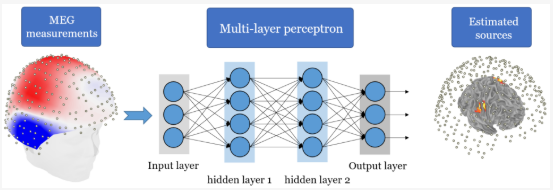
\includegraphics[scale=0.5]{figures/met/process.png}
    \caption{Ilustracion de la localizacion de fuentes MEG basado en modelo inverso\cite{Pantazis2021}}
    \label{fig:process}
\end{figure}

\subsubsection{Evaluación del Modelo}

La efectividad del modelo se evaluara utilizando métricas clásicas de clasificación como precisión, exactitud, sensibilidad, F1-score y matriz de confusión por clase (zona cerebral).



\section{Hipótesis}
Al entrenar un modelo inverso basado en redes neuronales profundas con datos EEG simulados, donde las ubicaciones de las fuentes neuronales son conocidas, es posible mejorar la precisión en la detección del origen de la señal cerebral. Este enfoque supera a métodos clásicos como MNE, sLORETA y VARETA en la estimación espacio-temporal de las fuentes.

\section{Objetivos}
\subsection{General}

Desarrollar un sistema basado en Deep Learning que permita localizar zonas activas cerebrales a partir de señales EEG preprocesadas, mediante un modelo inverso.

\subsection{Específicos}
\begin{enumerate}
    \item \textbf{Generación y Preprocesamiento de Señales EEG}

    Generar señales electroencefalográficas (EEG) artificiales correspondientes a la actividad cerebral relacionada con la activación de grupos musculares. Identificando segmentos de señal válidos que puedan ser utilizados para el análisis posterior.

    \item \textbf{Diseño y Entrenamiento del Modelo Inverso}

    Desarrollar un modelo inverso capaz de estimar la localización tridimensional de las fuentes neuronales responsables de las señales EEG registradas en la superficie del cuero cabelludo utilizando redes neuronales profundas. El desempeño del modelo será evaluado mediante pruebas controladas, incluyendo simulaciones con fuentes conocidas y validación cruzada con registros reales.

    \item \textbf{Identificación de Zonas de Activación Cerebral}

    Determinar las regiones corticales activas asociadas con la ejecución de tareas motoras específicas, comparando la localización estimada por el modelo con datos anatómicos y funcionales disponibles. 

    \item \textbf{Verificación la efectividad del modelo}

    Verificar la efectividad del modelo propuesto mediante métricas cuantitativas aplicadas a datos simulados y reales. Comparar datos de modelos existentes en igualdad de condiciones.
\end{enumerate}

\subsection{Cronograma}
\begin{landscape}
\begin{figure}%[H]
    \centering
    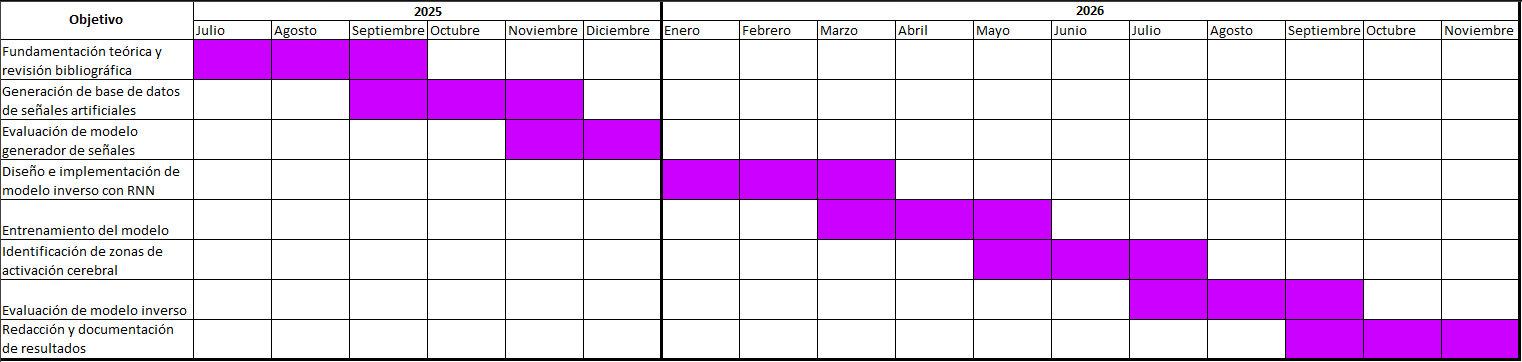
\includegraphics[scale=0.4]{figures/obj/cronograma.png}
    \caption{Cronograma de Actividades}
    \label{fig:crono}
\end{figure}
\end{landscape}

\section{Metodología}
    %\subsection{Metodología Propuesta}
    % 3-4 Pags

    \begin{figure}[H]
    \centering
    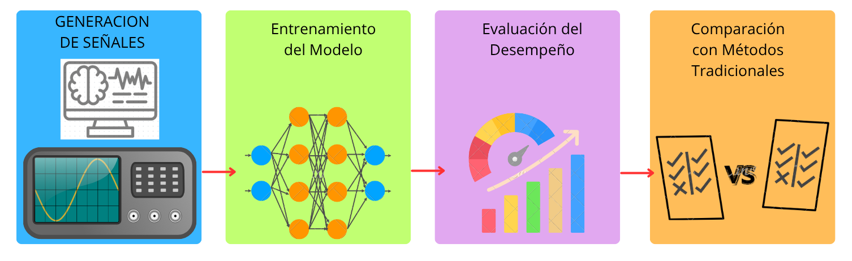
\includegraphics[scale=0.5]{figures/met/metodologia.png}
    \caption{Métodologia propuesta}
    \label{fig:met}
    \end{figure}

    Para abordar el problema inverso de localización de fuentes cerebrales a partir de señales EEG, se propone una metodología híbrida que integra modelos físicos de simulación, redes neuronales profundas y métricas de evaluación cuantitativa. Esta aproximación busca superar las limitaciones de los métodos clásicos mediante la incorporación de aprendizaje automático entrenado con datos simulados de alta fidelidad.

    \subsection{Generación de Datos Simulados}

    La primera etapa consiste en la creación de un conjunto de datos sintéticos que sirva como base de entrenamiento y validación del modelo. Para ello, se define un modelo de cabeza que representa las propiedades geométricas y de conductividad de los tejidos (cerebro, líquido cefalorraquídeo, cráneo y piel). Se consideran diferentes configuraciones, entre ellas:

    \begin{itemize}
    \item Modelo homogéneo: idealizado, de baja complejidad computacional.
    \item Método de elementos de frontera (BEM por sus siglas en inglés): solución numérica sobre mallas triangulares.
    \item Método de los Elementos Finitos (FEM por sus siglas en inglés): mayor precisión anatómica y flexibilidad geométrica.
    \item Modelo Localmente Esférico con Restricciones Anatómicas (LSMAC por sus siglas en inglés): aproximación esférica localmente adaptada a la anatomía.
    \end{itemize}

    El modelo de fuente define la distribución, orientación y dinámica temporal de los generadores neuronales. La actividad neuronal se modela mediante señales simples (como sinusoides) o patrones complejos generados con Neural Mass Models (NMMs), permitiendo simular potenciales evocados o actividad oscilatoria.

    Posteriormente, se resuelve el problema directo mediante el cálculo del lead field matrix, el cual permite proyectar la actividad de las fuentes a los sensores. A los datos generados se les añade ruido gaussiano controlado para simular condiciones reales.

    \subsection{Entrenamiento del Modelo de Deep Learning}

    Con los datos simulados se entrena una red neuronal profunda supervisada. La entrada del modelo consiste en señales EEG multicanal, y la salida corresponde a una estimación tridimensional de las fuentes activas. La arquitectura propuesta puede incluir:

    \begin{itemize}
        \item Redes convolucionales (CNN) para extracción de patrones espaciales.
        \item Redes recurrentes (RNN o LSTM) para capturar información temporal.
        \item Módulos de atención para mejorar la interpretación y localización.
    \end{itemize}

    El entrenamiento se realiza minimizando una función de pérdida compuesta por errores de localización y amplitud, con regularización para evitar sobreajuste.

    \subsection{Evaluación del Desempeño}

    Para validar la eficacia del modelo, se utilizarán métricas cuantitativas reconocidas en la literatura:

    \begin{itemize}
        \item \textbf{Localization Error (LE)}: distancia entre fuente estimada y real.
        \item \textbf{Temporal Error (TE)}: desviación entre los tiempos pico estimado y verdadero.
        \item \textbf{nMSE (Normalized Mean Squared Error)}: error cuadrático medio relativo.
        \item \textbf{PSNR (Peak Signal-to-Noise Ratio)}: calidad de la señal reconstruida.
        \item \textbf{Precision, Recall y F1-score}: para evaluar la detección correcta de regiones activas.
    \end{itemize}
    
    En el caso de datos reales, donde no se dispone de la “verdad conocida”, se utilizarán referencias clínicas como registros de iEEG o áreas de resección quirúrgica, así como comparación con modalidades complementarias como fMRI o PET.
    
    \subsection{Comparación con Métodos Tradicionales}
    
    Los resultados obtenidos serán comparados con los de técnicas clásicas de localización, como MNE, sLORETA y VARETA, utilizando el mismo conjunto de datos simulados y reales. Esta comparación permitirá establecer mejoras en términos de precisión espacial, temporal y robustez frente al ruido.


\subsection{Consideraciones Éticas}

Para el desarrollo de nuestro generador de señales así como la implementación de nuestro modelo se parte de bases de datos de EEG públicas de plataformas abiertas (como PhysioNet\cite{physionet2021auditoryeeg} o BNCI-Horizon 2020\cite{bnci2020datasets}). Las fuentes de estas bases de datos son abiertas y de uso libre para investigación por lo que no se requieren permisos o licencias especiales. Dado que esta información no recolecta información de fuentes primarias siendo datos de seres humanos no sera requerida consideraciones éticas extras. Las señales EEG utilizadas son datos públicos anonimizados y servirán exclusivamente como referencia para generar simulaciones sintéticas bajo condiciones controladas.


\section{Recursos}
Se deben describir los recursos que se usan en la investigación:

\begin{enumerate}
	\item Equipo de Computo:
	\begin{itemize}
		\item Nombre: LAPTOP-EHFPNJP6.
		\item Procesador	11th Gen Intel(R) Core(TM) i5-11400H @ 2.70GHz   2.69 GHz
		\item RAM instalada	16.0 GB (15.7 GB usable)
		\item Tipo de sistema	Sistema operativo de 64 bits, procesador basado en x64
	\end{itemize}

    \item Google Colaboratory (Colab)
    \begin{itemize}
        \item Plataforma de computación en la nube proporcionada por Google que permite ejecutar código Python en notebooks interactivos. Se emplea para el entrenamiento de modelos de deep learning, procesamiento de señales EEG y visualización de resultados. Facilita el acceso a recursos como GPU y TPU sin necesidad de instalación local.
    \end{itemize}
    
    \item BNCI Horizon 2020
    \begin{itemize}
    \item Repositorio público de conjuntos de datos EEG utilizado ampliamente en investigación en interfaces cerebro-computadora (BCI). Contiene datos anotados para tareas como imaginación motora, estados cognitivos y estímulos visuales o auditivos. 
    \item Enlace: \url{https://bnci-horizon-2020.eu/database/data-sets}
    \end{itemize}

    \item PhysioNet
    \begin{itemize}
    \item Plataforma que ofrece acceso abierto a datos fisiológicos, incluyendo EEG. El conjunto de datos \textit{Auditory EEG Dataset} contiene registros de respuesta cerebral a estímulos auditivos, útil para el análisis de procesamiento sensorial y cognitivo.
    \item Enlace: \url{https://physionet.org/content/auditory-eeg/1.0.0/}
\end{itemize}

\end{enumerate}


\section{Alcance del proyecto}
Este proyecto se enfoca en el desarrollo, entrenamiento y validación de un modelo inverso basado en redes neuronales profundas para la localización de fuentes neuronales a partir de señales EEG no invasivas. Se busca implementar la simulación de señales realistas mediante distintos modelos de cabeza (homogéneo, BEM, FEM) y la generación de actividad cerebral sintética con modelos biológicos como los Neural Mass Models.
    
Se entrenará un modelo de aprendizaje profundo (CNN y/o RNN) con estos datos, buscando estimar tanto la posición como la dinámica de las fuentes internas. El desempeño del modelo será evaluado cuantitativamente mediante métricas como el error de localización (LE), error temporal (TE), nMSE, PSNR, precisión, sensibilidad y F1-score. Además, se realizará una comparación sistemática con métodos clásicos como MNE, sLORETA y VARETA. 
    
También se contempla una validación cualitativa utilizando datos reales con base en evidencia clínica disponible y modalidades complementarias como fMRI o iEEG. No se incluyen en este proyecto la adquisición directa de datos en sujetos humanos ni procedimientos invasivos, enfocándose exclusivamente en simulaciones y el uso de datos estandarizados.


\section{Resultados esperados}
\begin{itemize}
    \item Mejorar la precisión espacial y temporal en la localización de fuentes neuronales a partir de señales EEG, en comparación con métodos tradicionales.
    \item Obtener una red neuronal profunda capaz de generalizar frente a distintas configuraciones de ruido, geometrías de cabeza y dinámicas de fuente.
    \item Reducir el error de localización (LE) y el error temporal (TE) en escenarios simulados.
    \item Aumentar las tasas de precisión y sensibilidad en la detección de zonas corticales activas.
    \item Validar cualitativamente la coherencia de los resultados estimados con hallazgos clínicos y modalidades complementarias (fMRI, iEEG).
\end{itemize}

\nocite{*} % Para mostrar todas las refencias sin citarlas
\renewcommand{\refname}{Referencias bibliográficas}
\printbibliography%
\end{document}